\documentclass{article}

% Math packages
\usepackage{amsmath}
\usepackage{amssymb}
\usepackage{float}

% R Table packages
% booktabs and float are used frequently by kableExtra output from R
\usepackage{booktabs}
\usepackage{float}
\usepackage{colortbl}
\usepackage{xcolor}

% Page layout libraries
\usepackage{a4wide}
\usepackage{setspace}
\usepackage{geometry}
%\usepackage{parskip}
\usepackage{fancyhdr}

% Setting up the heading style preferred here
\pagestyle{fancy}
\fancyhead[L]{\thepage}
\fancyhead[C]{}
\fancyhead[R]{\textrm{Robert Petit}}
\fancyfoot[L, C, R]{}


% this package helps us with including images. Setting the graphics path makes it easier to refer to things in the \includegraphics command.
\usepackage{graphicx}
\graphicspath{ {../Figures/} }

% And finally, continuing on my crusade to make Helvetica the universal standard
\usepackage[scaled]{helvet}
\renewcommand\familydefault{\sfdefault} 
\usepackage[T1]{fontenc}

% Titling
\title{Lott and Mustard Revisited}
\author{Robert Petit}
\date{May 2022}

\begin{document}
\maketitle

\section{Introduction}

The question of concealed carry permits and their effect on crimes has long been an extremely controversial topic. Lott and Mustard (1997) is an extremely important analysis of these permits but, since it's original publishing in 1997 research design has become far more adept at determining causal factors. 

By re-analyzing this data with newer, more thorough methods, we can investigate more closely the findings of the original paper and determine what, if any, effect these laws have on crime.

\section{Background and Theory}

Crime deterrence as a whole is a more-than controversial subject in the modern day; the concept of being "tough on crime" is commonplace in modern media and politics and comes in many forms, from increasing police presence and prison sentences to denying civil liberties and services in perpetuity. The goal is to drive the cost of crime so high that it becomes rare that a rational person would \emph{ever} choose to engage in illicit activity. "Shall-issue" laws are another step in this direction; these are state-level laws that ensure any person who is legal and meets some basic eligibility requirements be issued a permit for carrying a concealed weapon.

The theory here is quite simple: more armed victims \emph{should} mean a higher expected cost of committing a crime and, subsequently, a lower number of crimes committed. This carries the obvious restrictions that we would only expect this change in crimes where the victim is aware and present at the time the crime is committed, such as assault and robbery, and smaller or no changes when the victim is not present or aware, while the crime is being committed, such as auto theft. 

\begin{table}[H]

\caption{\label{tab:LawRollout}Shall-Issue Law Rollouts by State}
\centering
\begin{tabular}[t]{ll}
\toprule
State & Rollout\\
\midrule
\cellcolor{gray!6}{Alabama} & \cellcolor{gray!6}{Pre-1977}\\
Connecticut & Pre-1977\\
\cellcolor{gray!6}{Indiana} & \cellcolor{gray!6}{Pre-1977}\\
New Hampshire & Pre-1977\\
\cellcolor{gray!6}{North Dakota} & \cellcolor{gray!6}{Pre-1977}\\
\addlinespace
South Dakota & Pre-1977\\
\cellcolor{gray!6}{Vermont} & \cellcolor{gray!6}{Pre-1977}\\
Washington & Pre-1977\\
\cellcolor{gray!6}{Florida} & \cellcolor{gray!6}{1987}\\
Virginia & 1988\\
\addlinespace
\cellcolor{gray!6}{Georgia} & \cellcolor{gray!6}{1989}\\
Maine & 1989\\
\cellcolor{gray!6}{Oregon} & \cellcolor{gray!6}{1989}\\
Pennsylvania & 1989\\
\cellcolor{gray!6}{West Virginia} & \cellcolor{gray!6}{1989}\\
\addlinespace
Idaho & 1990\\
\cellcolor{gray!6}{Mississipi} & \cellcolor{gray!6}{1990}\\
Montana & 1991\\
\bottomrule
\end{tabular}
\end{table}


Shall-issue laws were a hot-bed political topic starting in 1976 and, from 1987 to 1991
\footnote{The years for each law come from Lott and Mustard (1997) \cite{LottMustard} and Cramer and Kopel (1995) \cite{CramerKopel}. The only discrepancy between the two sources is that of Oregon, which Lott and Mustard list as 1990 whereas Cramer and Kopel cite the law as 1989. This may be due to the timing of the law, later analysis does not seem consequentially sensitive to this shift in any case.}
there were several of these laws passed. Prior to this wave of laws (and the start of our data) there were eight states that already had these laws in effect. These laws were very similar to one another in that they funcitonally removed the ability for any lower-than-state level official to restrict the issuance of a gun permit. There is some heterogeneity among the effect of these laws within each state, since some officials were more restrictive than others, but across each state this resulted in greater access to concealed carry permits issuance.

We will use several models to determine the effect of these laws on crimes; our goal here is to determine the average treatment effect on the treated groups. The model most similar to the approach of Lott and Mustard (1997) \cite{LottMustard} is the two-way fixed effect model but this estimator is known to have some unfavorable properties. To handle this, we will also investigate the Bacon decomposition \cite{Bacon} for the two-way fixed effect model.  Implement the Callaway and Sant'anna estimator \cite{CallawaySantanna} and the Sun and Abraham event study to get a more contemporary idea of the effects.

\section{Data}

Here we are working with the state level data from the National Research Council's review of firearms and gun violence, provided by Peter Donohue \cite{Donohue}. This data covers the yearly crimes for violent crimes and property crimes in all fifty states from 1977 to 2006. The violent crimes subdivided into murder, rape, assault and the property crimes are subdivided into robbery, auto theft, burglary, and larceny.

\begin{table}[!h]

\caption{\label{tab:CrimeSummary}Summary Statistics for Statewide Yearly Crimes and Crime Rates}
\centering
\begin{tabular}[t]{lrrr}
\toprule
Variable & N. Obs & Mean & Std. Dev\\
\midrule
\addlinespace[0.3em]
\multicolumn{4}{l}{\textbf{Crime Counts}}\\
\hspace{1em}\cellcolor{gray!6}{Violent Crimes} & \cellcolor{gray!6}{1941} & \cellcolor{gray!6}{27066.81} & \cellcolor{gray!6}{41920.33}\\
\hspace{1em}Property Crimes & 1941 & 211212.22 & 262156.25\\
\hspace{1em}\cellcolor{gray!6}{Murder} & \cellcolor{gray!6}{1941} & \cellcolor{gray!6}{382.63} & \cellcolor{gray!6}{529.34}\\
\hspace{1em}Rape & 1941 & 1631.25 & 2054.90\\
\hspace{1em}\cellcolor{gray!6}{Assault} & \cellcolor{gray!6}{1941} & \cellcolor{gray!6}{15421.66} & \cellcolor{gray!6}{23517.30}\\
\hspace{1em}Robbery & 1941 & 9631.27 & 17207.33\\
\hspace{1em}\cellcolor{gray!6}{Auto Theft} & \cellcolor{gray!6}{1941} & \cellcolor{gray!6}{23714.54} & \cellcolor{gray!6}{37503.03}\\
\hspace{1em}Burglary & 1941 & 54414.24 & 72421.71\\
\hspace{1em}\cellcolor{gray!6}{Larceny} & \cellcolor{gray!6}{1941} & \cellcolor{gray!6}{133083.69} & \cellcolor{gray!6}{157018.36}\\
\addlinespace[0.3em]
\multicolumn{4}{l}{\textbf{Crime Rates}}\\
\hspace{1em}Violent Crime Rate & 1941 & 458.85 & 309.28\\
\hspace{1em}\cellcolor{gray!6}{Property Crime Rate} & \cellcolor{gray!6}{1941} & \cellcolor{gray!6}{4168.46} & \cellcolor{gray!6}{1256.21}\\
\hspace{1em}Murder Rate & 1941 & 7.25 & 6.80\\
\hspace{1em}\cellcolor{gray!6}{Rape Rate} & \cellcolor{gray!6}{1941} & \cellcolor{gray!6}{32.33} & \cellcolor{gray!6}{14.52}\\
\hspace{1em}Assault Rate & 1941 & 270.80 & 167.23\\
\hspace{1em}\cellcolor{gray!6}{Robbery Rate} & \cellcolor{gray!6}{1941} & \cellcolor{gray!6}{148.48} & \cellcolor{gray!6}{160.60}\\
\hspace{1em}Auto Theft Rate & 1941 & 404.60 & 234.87\\
\hspace{1em}\cellcolor{gray!6}{Burglary Rate} & \cellcolor{gray!6}{1941} & \cellcolor{gray!6}{1046.53} & \cellcolor{gray!6}{429.72}\\
\hspace{1em}Larceny Rate & 1941 & 2717.34 & 788.57\\
\bottomrule
\end{tabular}
\end{table}




\section{Empirical Models}

We need to visit two separate models, the first is a standard two-way fixed effect model as was carried out in Lott and Mustard (2017). For our purposes, we will still be using the state level data, and we will specifically look at the Bacon decomposition to consider the potential innaccuracies of this model.

Following that, we will look at the Callaway Sant'anna estimation, which will avoid the unfavorable properties of the two-way fixed effect model, and look at the effects in the form of an event study.

\subsection{Two-Way Fixed Effects}

This model is estimated by regressing the natural log of crime rates on the treatment, as well as the arrest rate for that specific crime. This provides an estimation of change in crime in terms of percentages, controlling for the current level of enforcement. We also include a wide variety of controls for demographic shifts over time.


\begingroup
\centering
\begin{tabular}{lcccc}
   \tabularnewline \midrule \midrule
   Dependent Variables: & Violent  & Murder   & Rape            & Assault\\  
   Model:               & (1)      & (2)      & (3)             & (4)\\  
   \midrule
   \emph{Variables}\\
   Treatment            & -0.0505  & -0.0280  & -0.0878$^{***}$ & -0.0403\\   
                        & (0.0367) & (0.0341) & (0.0308)        & (0.0508)\\   
   \midrule
   \emph{Fixed-effects}\\
   year                 & Yes      & Yes      & Yes             & Yes\\  
   fipsstat             & Yes      & Yes      & Yes             & Yes\\  
   \midrule
   \emph{Fit statistics}\\
   Observations         & 1,481    & 1,436    & 1,429           & 1,439\\  
   R$^2$                & 0.95783  & 0.93192  & 0.88324         & 0.92972\\  
   Within R$^2$         & 0.34949  & 0.23081  & 0.50501         & 0.26237\\  
   \midrule \midrule
   \multicolumn{5}{l}{\emph{Clustered (year \& fipsstat) standard-errors in parentheses}}\\
   \multicolumn{5}{l}{\emph{Signif. Codes: ***: 0.01, **: 0.05, *: 0.1}}\\
\end{tabular}
\par\endgroup



\begingroup
\centering
\begin{tabular}{lcccc}
   \tabularnewline \midrule \midrule
   Dependent Variables: & Violent  & Murder   & Rape            & Assault\\  
   Model:               & (1)      & (2)      & (3)             & (4)\\  
   \midrule
   \emph{Variables}\\
   Treatment            & -0.0505  & -0.0280  & -0.0878$^{***}$ & -0.0403\\   
                        & (0.0367) & (0.0341) & (0.0308)        & (0.0508)\\   
   \midrule
   \emph{Fixed-effects}\\
   year                 & Yes      & Yes      & Yes             & Yes\\  
   fipsstat             & Yes      & Yes      & Yes             & Yes\\  
   \midrule
   \emph{Fit statistics}\\
   Observations         & 1,481    & 1,436    & 1,429           & 1,439\\  
   R$^2$                & 0.95783  & 0.93192  & 0.88324         & 0.92972\\  
   Within R$^2$         & 0.34949  & 0.23081  & 0.50501         & 0.26237\\  
   \midrule \midrule
   \multicolumn{5}{l}{\emph{Clustered (year \& fipsstat) standard-errors in parentheses}}\\
   \multicolumn{5}{l}{\emph{Signif. Codes: ***: 0.01, **: 0.05, *: 0.1}}\\
\end{tabular}
\par\endgroup





\begingroup
\centering
\begin{tabular}{lccccc}
   \tabularnewline \midrule \midrule
   Dependent Variables: & Property & Robbery       & Auto     & Burglary & Larceny\\  
   Model:               & (1)      & (2)           & (3)      & (4)      & (5)\\  
   \midrule
   \emph{Variables}\\
   Treatment            & 0.0205   & -0.0490$^{*}$ & 0.0464   & -0.0277  & 0.0281\\   
                        & (0.0159) & (0.0274)      & (0.0435) & (0.0205) & (0.0169)\\   
   \midrule
   \emph{Fixed-effects}\\
   year                 & Yes      & Yes           & Yes      & Yes      & Yes\\  
   fipsstat             & Yes      & Yes           & Yes      & Yes      & Yes\\  
   \midrule
   \emph{Fit statistics}\\
   Observations         & 1,489    & 1,436         & 1,438    & 1,439    & 1,439\\  
   R$^2$                & 0.93649  & 0.97382       & 0.91642  & 0.94993  & 0.92891\\  
   Within R$^2$         & 0.59052  & 0.42838       & 0.52291  & 0.56501  & 0.57558\\  
   \midrule \midrule
   \multicolumn{6}{l}{\emph{Clustered (year \& fipsstat) standard-errors in parentheses}}\\
   \multicolumn{6}{l}{\emph{Signif. Codes: ***: 0.01, **: 0.05, *: 0.1}}\\
\end{tabular}
\par\endgroup



\begingroup
\centering
\begin{tabular}{lccccc}
   \tabularnewline \midrule \midrule
   Dependent Variables: & Property & Robbery       & Auto     & Burglary & Larceny\\  
   Model:               & (1)      & (2)           & (3)      & (4)      & (5)\\  
   \midrule
   \emph{Variables}\\
   Treatment            & 0.0205   & -0.0490$^{*}$ & 0.0464   & -0.0277  & 0.0281\\   
                        & (0.0159) & (0.0274)      & (0.0435) & (0.0205) & (0.0169)\\   
   \midrule
   \emph{Fixed-effects}\\
   year                 & Yes      & Yes           & Yes      & Yes      & Yes\\  
   fipsstat             & Yes      & Yes           & Yes      & Yes      & Yes\\  
   \midrule
   \emph{Fit statistics}\\
   Observations         & 1,489    & 1,436         & 1,438    & 1,439    & 1,439\\  
   R$^2$                & 0.93649  & 0.97382       & 0.91642  & 0.94993  & 0.92891\\  
   Within R$^2$         & 0.59052  & 0.42838       & 0.52291  & 0.56501  & 0.57558\\  
   \midrule \midrule
   \multicolumn{6}{l}{\emph{Clustered (year \& fipsstat) standard-errors in parentheses}}\\
   \multicolumn{6}{l}{\emph{Signif. Codes: ***: 0.01, **: 0.05, *: 0.1}}\\
\end{tabular}
\par\endgroup




In this estimation, we find that there is a small but statistically insignificant reduction in violent crime. The only specific crime that has a significant reduction is rape, which drops by a surprising 8.8\%. 

On the flip side, we see a slight but insignificant increase in property crimes, with a somewhat-significant increase in robbery specifically. This is not inconsistent with, but is far less decisive than, the results found by Lott and Mustard, where there is a reduction in violent crime and a smaller increase in property crime.

\subsection{Bacon Decomposition}

When estimating the weights and average estimates of the treatment variables, there are some obvious issues that arise. The Earlier vs. Later treated group has an outsized weight compared to the other groups, while the Later vs. Earlier treated group is much smaller. 

\begin{table}[!h]

\caption{\label{tab:BDec}Bacon Decomposition}
\centering
\begin{tabular}[t]{lrr}
\toprule
Type & Weight & Average Est\\
\midrule
\cellcolor{gray!6}{Earlier vs Later Treated} & \cellcolor{gray!6}{0.2742302} & \cellcolor{gray!6}{0.0021544}\\
Later vs Always Treated & 0.2351916 & 0.0574595\\
\cellcolor{gray!6}{Later vs Earlier Treated} & \cellcolor{gray!6}{0.0873926} & \cellcolor{gray!6}{0.0446130}\\
Treated vs Untreated & 0.4031856 & 0.1965715\\
\bottomrule
\end{tabular}
\end{table}


Principally, these group weightings can cause our estimates to be inconsistent to the point of uselessness, especially in situations where there are already-strong trends year over year, and comparing a treated group to a treated group in this case can cause wildly inconsistent estimations.

\subsection{Callaway and Sant'Anna}

For a more accurate estimation in which we never compare a treated group to another treated group, we can turn to Callaway and Sant'Anna \cite{CallawaySantanna}. For this estimation, we will look at the treatment for all states in a single year as a collective and look at the treatment effect for those states. We will narrow our focus to violent crimes for now, since these are the crimes where we will find conclusive results, if there are any. 

\begin{table}[!h]

\caption{\label{tab:CSEst}Aggregate Group ATTs}
\centering
\begin{tabular}[t]{rrr}
\toprule
Group & Aggregate ATT & SE\\
\midrule
\cellcolor{gray!6}{1977} & \cellcolor{gray!6}{-6969.74} & \cellcolor{gray!6}{3139.42}\\
1987 & 18177.69 & 1345.91\\
\cellcolor{gray!6}{1988} & \cellcolor{gray!6}{2460.28} & \cellcolor{gray!6}{1543.74}\\
1989 & 1665.33 & 2524.69\\
\cellcolor{gray!6}{1990} & \cellcolor{gray!6}{2383.97} & \cellcolor{gray!6}{2455.67}\\
\addlinespace
1991 & 6747.73 & 3142.71\\
\bottomrule
\end{tabular}
\end{table}


Here, the estimation is *far* different; the average treatment effect on the treated group is barely negative, and only significantly so for the very first group of treated states. In no case do we have conclusive evidence that these crimes are being influenced much at all.

\subsection{Event Study}

Considering this data in the form of an event study, where we aggregate the effects by the years since the treatment for each group; negative values are the pre-treatment years, in which we can see both the trends and potentially anticipation. Our pre-treatment 'trend difference' provides some intuition of the potential accuracy we could attain from our data set. The post-event estimations fail to show any conclusive evidence that there are effects on the violent crime rate from these laws. We also see extremely wide standard errors and a noisy estimation in general, both of which indicate that there is very little to be pulled from this data set beyond simply failing to reject the null hypothesis that more guns means nothing for crime.

\begin{table}

\caption{\label{tab:SAEst}Event Study}
\centering
\begin{tabular}[t]{rrrrr}
\toprule
\multicolumn{3}{c}{ } & \multicolumn{2}{c}{95\% Confidence Interval} \\
\cmidrule(l{3pt}r{3pt}){4-5}
Event Time & Coefficient & SE & Lower & Upper\\
\midrule
\cellcolor{gray!6}{-5} & \cellcolor{gray!6}{-0.0481866} & \cellcolor{gray!6}{0.1873409} & \cellcolor{gray!6}{-0.4153679} & \cellcolor{gray!6}{0.3189948}\\
-4 & -0.0075730 & 0.1867580 & -0.3736120 & 0.3584661\\
\cellcolor{gray!6}{-3} & \cellcolor{gray!6}{-0.0525203} & \cellcolor{gray!6}{0.2112834} & \cellcolor{gray!6}{-0.4666282} & \cellcolor{gray!6}{0.3615875}\\
-2 & -0.0012044 & 0.2371528 & -0.4660153 & 0.4636066\\
\cellcolor{gray!6}{-1} & \cellcolor{gray!6}{0.0250265} & \cellcolor{gray!6}{0.2434649} & \cellcolor{gray!6}{-0.4521559} & \cellcolor{gray!6}{0.5022090}\\
\addlinespace
0 & -0.0380029 & 0.2470897 & -0.5222897 & 0.4462840\\
\cellcolor{gray!6}{1} & \cellcolor{gray!6}{-0.0388197} & \cellcolor{gray!6}{0.2408278} & \cellcolor{gray!6}{-0.5108336} & \cellcolor{gray!6}{0.4331942}\\
2 & -0.0634309 & 0.2342575 & -0.5225671 & 0.3957053\\
\cellcolor{gray!6}{3} & \cellcolor{gray!6}{-0.0639702} & \cellcolor{gray!6}{0.2248330} & \cellcolor{gray!6}{-0.5046348} & \cellcolor{gray!6}{0.3766944}\\
4 & -0.0963113 & 0.2402981 & -0.5672869 & 0.3746644\\
\addlinespace
\cellcolor{gray!6}{5} & \cellcolor{gray!6}{-0.0619916} & \cellcolor{gray!6}{0.2230570} & \cellcolor{gray!6}{-0.4991752} & \cellcolor{gray!6}{0.3751921}\\
6 & -0.0900063 & 0.2353931 & -0.5513684 & 0.3713557\\
\cellcolor{gray!6}{7} & \cellcolor{gray!6}{-0.0069768} & \cellcolor{gray!6}{0.2452190} & \cellcolor{gray!6}{-0.4875971} & \cellcolor{gray!6}{0.4736436}\\
8 & 0.0214361 & 0.2370008 & -0.4430769 & 0.4859491\\
\cellcolor{gray!6}{9} & \cellcolor{gray!6}{0.0922565} & \cellcolor{gray!6}{0.2267394} & \cellcolor{gray!6}{-0.3521445} & \cellcolor{gray!6}{0.5366575}\\
\addlinespace
10 & 0.1634692 & 0.2114618 & -0.2509882 & 0.5779267\\
\bottomrule
\end{tabular}
\end{table}


\begin{figure}[H]
    \begin{center}
        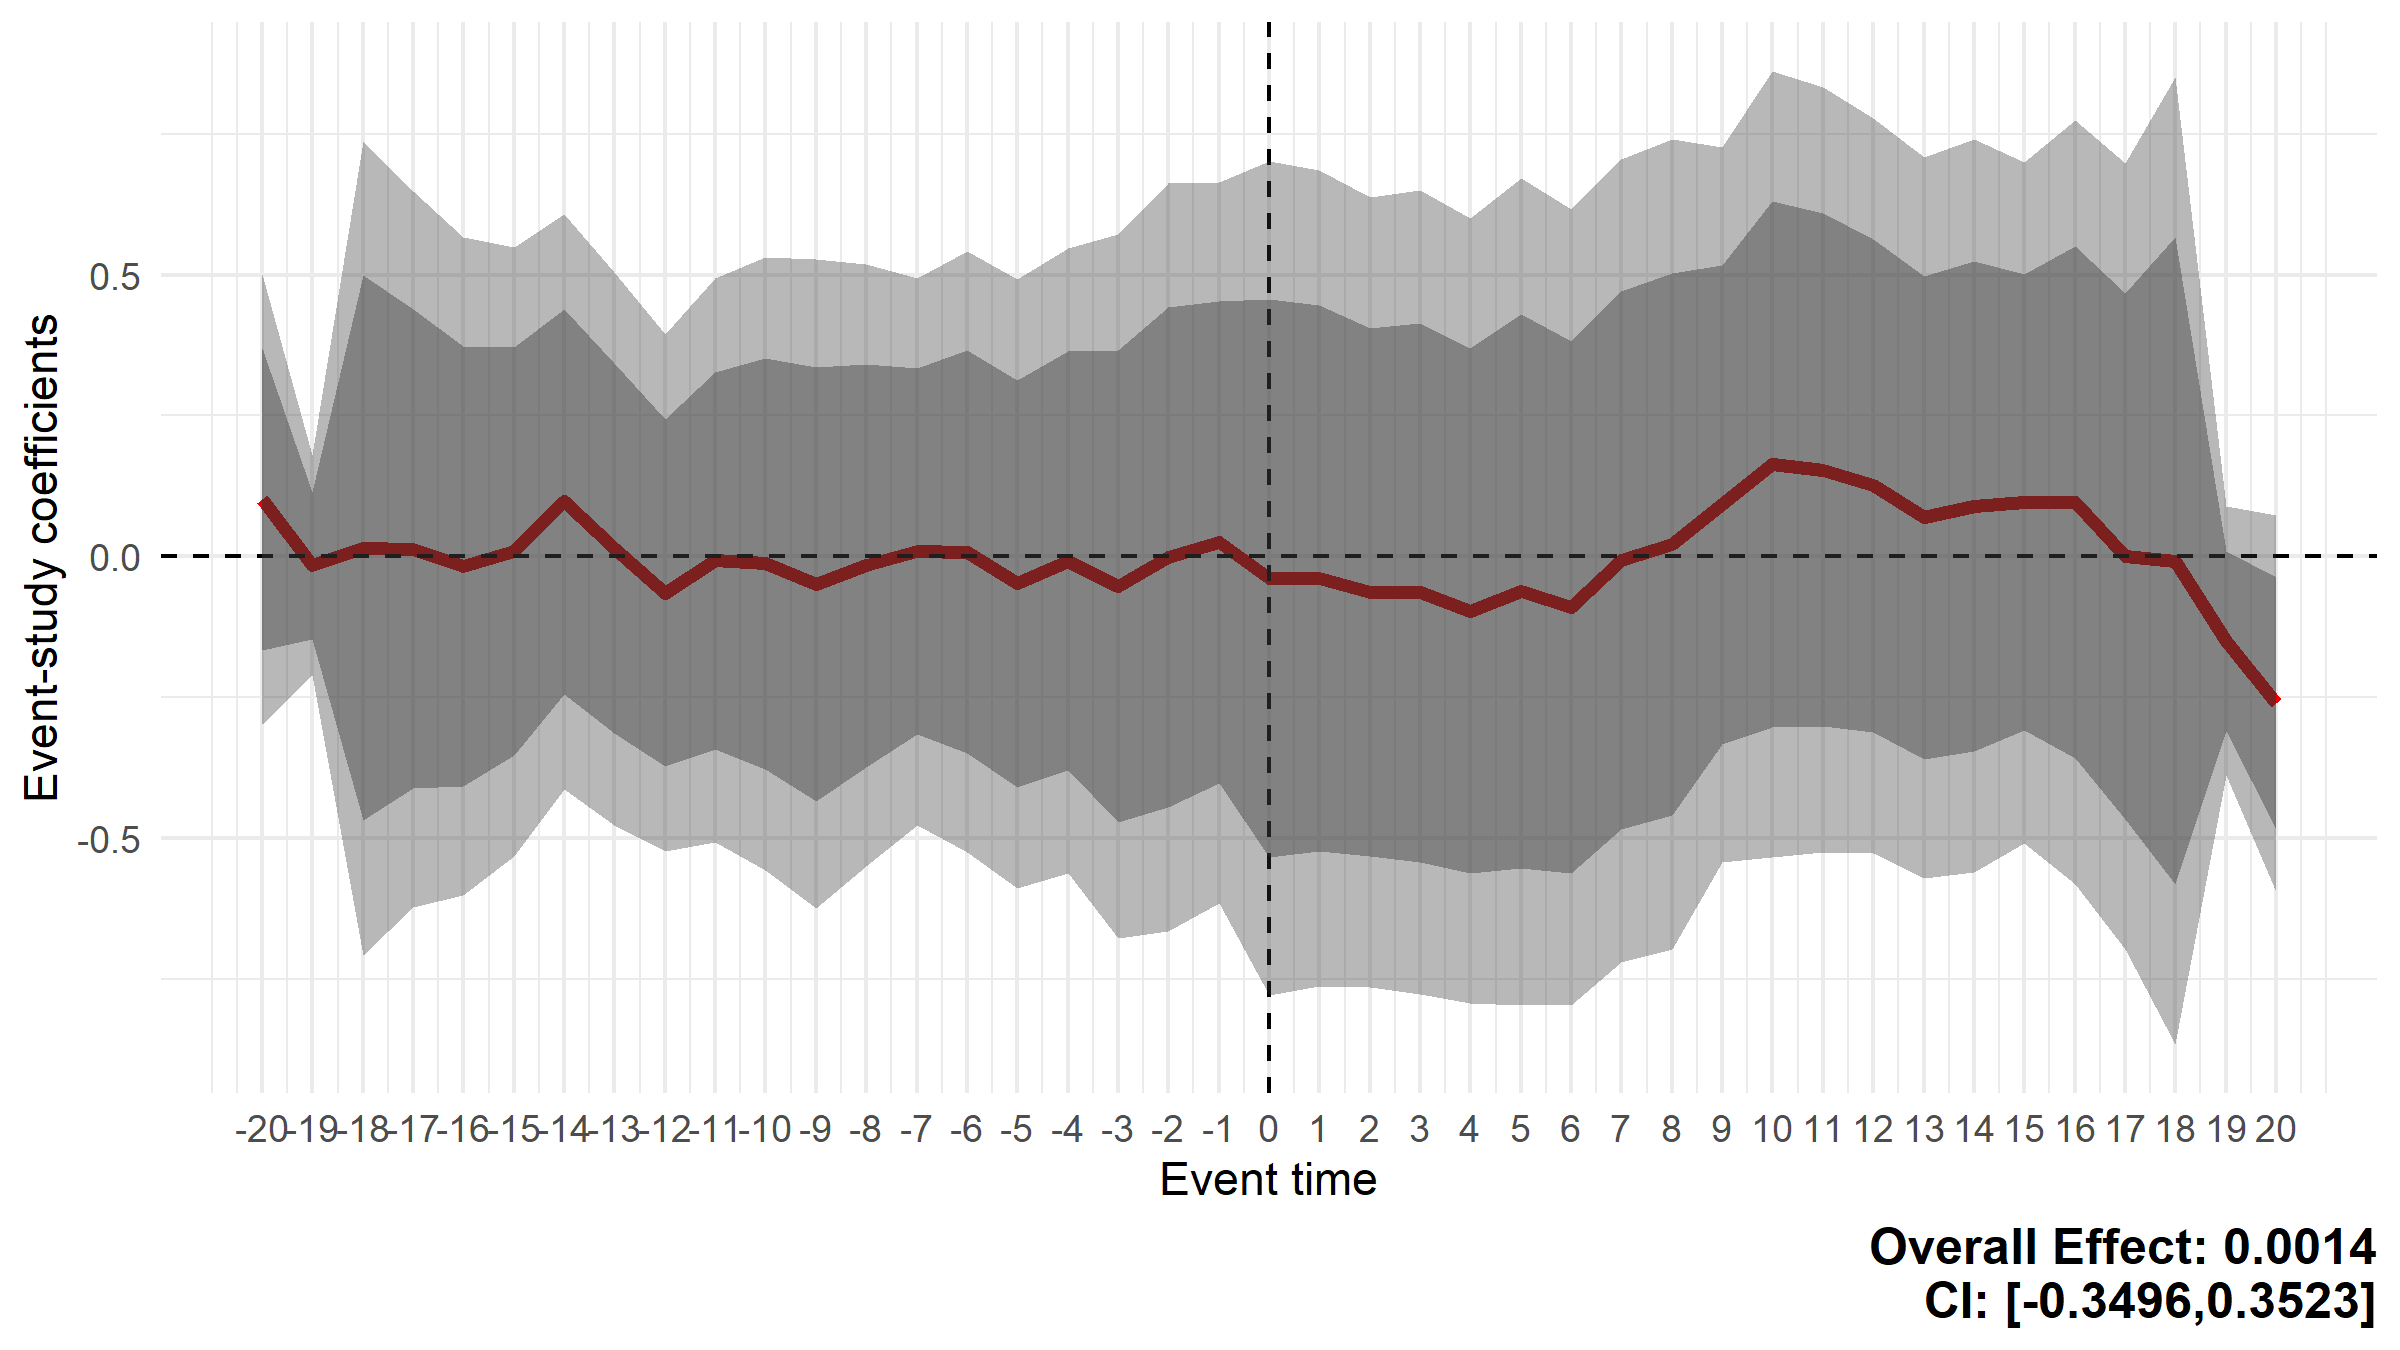
\includegraphics[width=.85\textwidth]{SA_EventStudy.png}
    \end{center}
    \caption{Event Study of Shall Issue law passage}
    \label{fig:ESFig}
\end{figure}

\subsection*{Full Callaway Sant'Anna Results}

The analysis of the violent crime trends continues to hold when we observe  crimes for which we have data.

\begin{table}[!h]

\caption{\label{tab:CSEst}Aggregate Group ATTs, Violent Crimes}
\centering
\begin{tabular}[t]{rrrrrrrrr}
\toprule
\multicolumn{1}{c}{ } & \multicolumn{2}{c}{Violent} & \multicolumn{2}{c}{Murder} & \multicolumn{2}{c}{Rape} & \multicolumn{2}{c}{Assault} \\
\cmidrule(l{3pt}r{3pt}){2-3} \cmidrule(l{3pt}r{3pt}){4-5} \cmidrule(l{3pt}r{3pt}){6-7} \cmidrule(l{3pt}r{3pt}){8-9}
Group & ATT & SE & ATT & SE & ATT & SE & ATT & SE\\
\midrule
\cellcolor{gray!6}{1987} & \cellcolor{gray!6}{-0.13} & \cellcolor{gray!6}{0.08} & \cellcolor{gray!6}{-0.33} & \cellcolor{gray!6}{0.04} & \cellcolor{gray!6}{-0.17} & \cellcolor{gray!6}{0.04} & \cellcolor{gray!6}{-0.05} & \cellcolor{gray!6}{0.03}\\
1988 & 0.01 & 0.08 & 0.01 & 0.04 & -0.02 & 0.04 & 0.02 & 0.03\\
\cellcolor{gray!6}{1989} & \cellcolor{gray!6}{-0.03} & \cellcolor{gray!6}{0.31} & \cellcolor{gray!6}{-0.21} & \cellcolor{gray!6}{0.11} & \cellcolor{gray!6}{-0.06} & \cellcolor{gray!6}{0.10} & \cellcolor{gray!6}{0.02} & \cellcolor{gray!6}{0.19}\\
1990 & 0.03 & 0.09 & 0.15 & 0.03 & 0.32 & 0.04 & -0.04 & 0.03\\
\cellcolor{gray!6}{1991} & \cellcolor{gray!6}{0.48} & \cellcolor{gray!6}{0.09} & \cellcolor{gray!6}{-0.36} & \cellcolor{gray!6}{0.04} & \cellcolor{gray!6}{0.20} & \cellcolor{gray!6}{0.03} & \cellcolor{gray!6}{0.55} & \cellcolor{gray!6}{0.03}\\
\bottomrule
\end{tabular}
\end{table}


\begin{table}[!h]

\caption{\label{tab:CSEst}Aggregate Group ATTs, Property Crimes}
\centering
\begin{tabular}[t]{rrrrrrrrrrr}
\toprule
\multicolumn{1}{c}{ } & \multicolumn{2}{c}{Property} & \multicolumn{2}{c}{Robery} & \multicolumn{2}{c}{Auto} & \multicolumn{2}{c}{Burglary} & \multicolumn{2}{c}{Larceny} \\
\cmidrule(l{3pt}r{3pt}){2-3} \cmidrule(l{3pt}r{3pt}){4-5} \cmidrule(l{3pt}r{3pt}){6-7} \cmidrule(l{3pt}r{3pt}){8-9} \cmidrule(l{3pt}r{3pt}){10-11}
Group & ATT & SE & ATT & SE & ATT & SE & ATT & SE & ATT & SE\\
\midrule
\cellcolor{gray!6}{1987} & \cellcolor{gray!6}{-0.10} & \cellcolor{gray!6}{0.03} & \cellcolor{gray!6}{-0.28} & \cellcolor{gray!6}{0.04} & \cellcolor{gray!6}{0.00} & \cellcolor{gray!6}{0.05} & \cellcolor{gray!6}{-0.12} & \cellcolor{gray!6}{0.03} & \cellcolor{gray!6}{-0.09} & \cellcolor{gray!6}{0.02}\\
1988 & 0.02 & 0.02 & 0.02 & 0.04 & -0.02 & 0.05 & -0.07 & 0.03 & 0.04 & 0.02\\
\cellcolor{gray!6}{1989} & \cellcolor{gray!6}{0.02} & \cellcolor{gray!6}{0.06} & \cellcolor{gray!6}{-0.14} & \cellcolor{gray!6}{0.14} & \cellcolor{gray!6}{-0.17} & \cellcolor{gray!6}{0.10} & \cellcolor{gray!6}{-0.03} & \cellcolor{gray!6}{0.09} & \cellcolor{gray!6}{0.06} & \cellcolor{gray!6}{0.06}\\
1990 & 0.00 & 0.02 & 0.25 & 0.04 & 0.19 & 0.06 & -0.03 & 0.02 & -0.01 & 0.02\\
\cellcolor{gray!6}{1991} & \cellcolor{gray!6}{0.01} & \cellcolor{gray!6}{0.02} & \cellcolor{gray!6}{0.28} & \cellcolor{gray!6}{0.04} & \cellcolor{gray!6}{0.03} & \cellcolor{gray!6}{0.06} & \cellcolor{gray!6}{-0.11} & \cellcolor{gray!6}{0.03} & \cellcolor{gray!6}{0.01} & \cellcolor{gray!6}{0.02}\\
\bottomrule
\end{tabular}
\end{table}


You can still see very clearly that there are no substantial effects beyond the very slightest effect in the first year estimated. Even those effects are only minimally significant.

\section{Conclusion}

From this we can handily conclude that the effect of shall issue laws on crime are not statistically significant or substantial. This is a partial refutation of the conclusions in Lott and Mustard (2017), though Lott and Mustard use the slightly-different county level data.

There is one factor in this analysis that is a complete mismatch with the original data: the within state heterogeneity in the impact of these laws is unaccounted for in this state level data. This may be non-trivial but, since these laws are passed at the state level, the aggregate effect of these laws should be evaluated at the state level. 

Regardless, given the slight differences between the state-level and county-level analysis and the similarity between the state- and county-level Bacon Decomposition, it is likely that the bias implicit in a two way fixed effect model is also similiar.


\bibliography{LottMustardReplication_Bib}
\bibliographystyle{plain}

\end{document}